% Asset ID: A22ProjectilesTikZ-005
% Purpose: Derivation map for projectile formulae.
\documentclass[tikz,border=8pt]{standalone}
\usepackage{amsmath}
\usetikzlibrary{arrows.meta,positioning}
\begin{document}
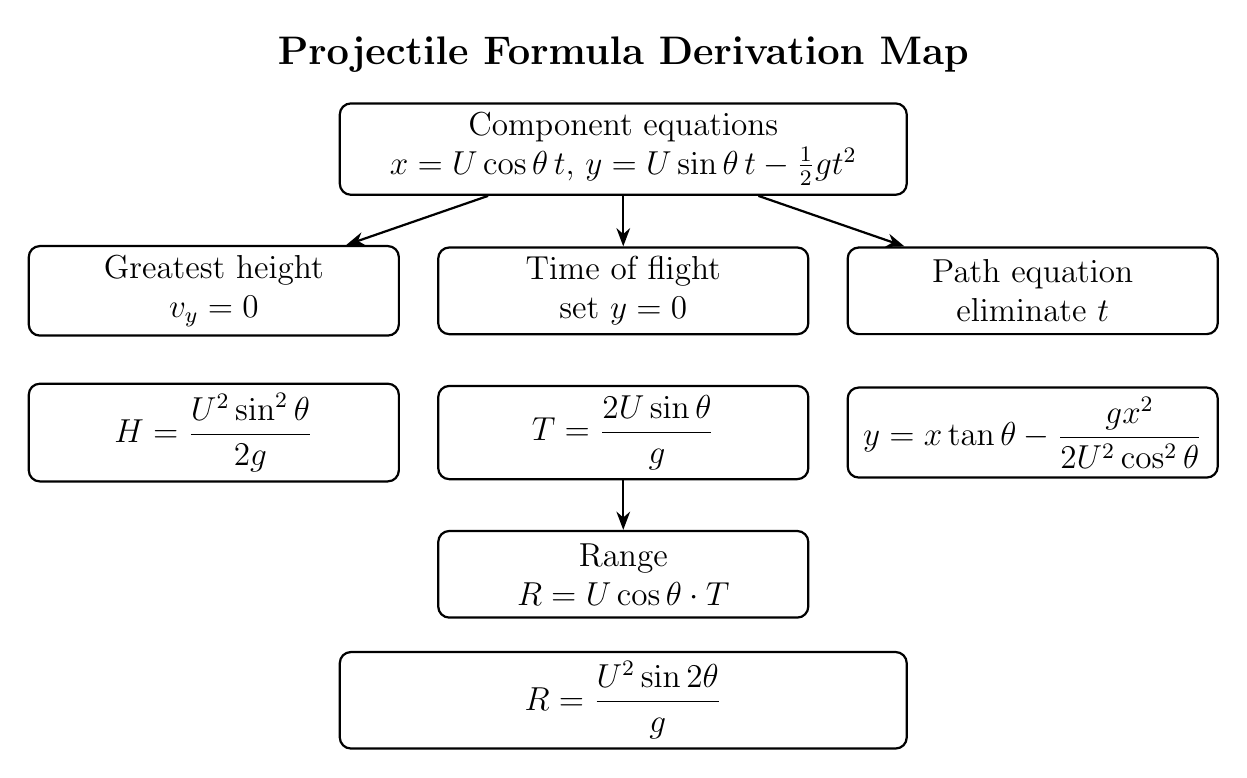
\begin{tikzpicture}[>=Stealth,box/.style={draw,rounded corners,thick,align=center,font=\large,minimum width=4.7cm,minimum height=1.1cm},widebox/.style={draw,rounded corners,thick,align=center,font=\large,minimum width=7.2cm,minimum height=1.15cm},arrow/.style={->,thick},title/.style={font=\Large\bfseries}]
\node[title] at (0,4.6) {Projectile Formula Derivation Map};
\node[widebox] (start) at (0,3.4) {Component equations\\$x=U\cos\theta\,t$, $y=U\sin\theta\,t-\frac12gt^2$};
\node[box] (height) at (-5.2,1.6) {Greatest height\\$v_y=0$}; \node[box] (time) at (0,1.6) {Time of flight\\set $y=0$}; \node[box] (path) at (5.2,1.6) {Path equation\\eliminate $t$};
\draw[arrow] (start)--(height); \draw[arrow] (start)--(time); \draw[arrow] (start)--(path);
\node[box] at (-5.2,-0.2) {$H=\dfrac{U^2\sin^2\theta}{2g}$};
\node[box] (tformula) at (0,-0.2) {$T=\dfrac{2U\sin\theta}{g}$};
\node[box] at (5.2,-0.2) {$y=x\tan\theta-\dfrac{gx^2}{2U^2\cos^2\theta}$};
\node[box] (range) at (0,-2.0) {Range\\$R=U\cos\theta \cdot T$}; \node[widebox] at (0,-3.6) {$R=\dfrac{U^2\sin2\theta}{g}$};
\draw[arrow] (tformula)--(range);
\end{tikzpicture}
\end{document}
